\begin{frame}{Fine-Tuning Can Cost Accuracy Under Shift}
  \begin{columns}[T,onlytextwidth]
    \column{0.42\textwidth}
      \begin{itemize}\footnotesize\itemsep0.3em
        \item \textbf{Distribution shift} in this section: covariate shift (covered earlier), the same classes in a new image style or source.
        \item \textbf{ID} (in-distribution) accuracy: on the distribution used for fine-tuning. \textbf{OOD} (out-of-distribution) accuracy: on shifted test sets with the same classes.
        \item ImageNet-R holds renditions such as paintings and sculptures; ImageNet-A holds natural images that a ResNet-50 misclassifies.
      \end{itemize}
    \column{0.56\textwidth}
      \centering
      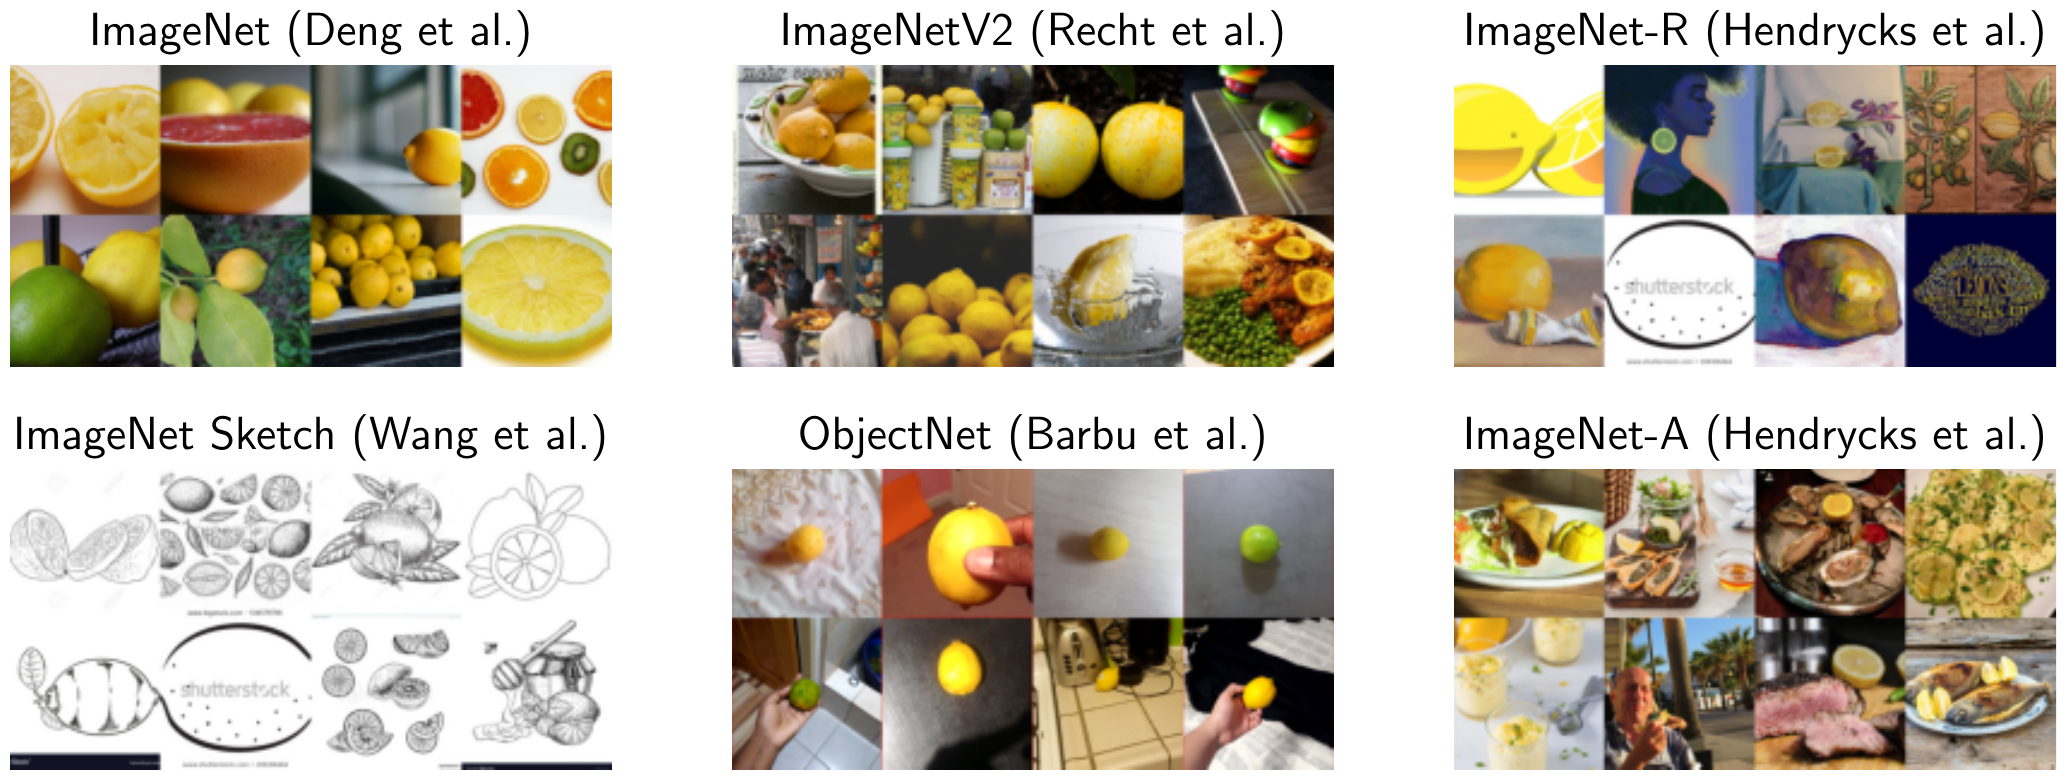
\includegraphics[width=\linewidth,height=0.50\textheight,keepaspectratio]{images/image-recognition/wiseft_fig2_lemon_shift_datasets.png}\\[0.2em]
      {\scriptsize Samples of the class lemon from ImageNet and five shifted test sets. Wortsman et al., ``Robust fine-tuning of zero-shot models,'' CVPR 2022, \href{https://arxiv.org/abs/2109.01903v3}{arXiv:2109.01903v3}, Figure~2.\par}
  \end{columns}
  \vspace{0.3em}
  \begin{itemize}\footnotesize
    \item Zero-shot CLIP holds up well under shift (covered earlier). Fine-tuning it end-to-end on ImageNet gains 9.6 points there and loses 4.8 points of mean shift accuracy:
  \end{itemize}
  \vspace{0.1em}
  {\centering\scriptsize\setlength{\tabcolsep}{4pt}
  \begin{tabular}{l c c c c c c c}
    \toprule
    CLIP ViT-L/14@336px & IN & IN-V2 & IN-R & IN-Sketch & ObjectNet & IN-A & Mean, 5 shifts \\
    \midrule
    Zero-shot & 76.6 & 70.5 & 89.0 & 60.9 & 69.1 & 77.7 & 73.4 \\
    Fine-tuned end-to-end & 86.2 & 76.8 & 79.8 & 57.9 & 63.3 & 65.4 & 68.6 \\
    \bottomrule
  \end{tabular}\par}
  \vspace{0.15em}
  {\centering\scriptsize Top-1 accuracy (\%); IN: ImageNet. Wortsman et al., \href{https://arxiv.org/abs/2109.01903v3}{arXiv:2109.01903v3}, Table~1.\par}
\end{frame}

\begin{frame}{LP-FT: Linear Probe First, Then Fine-Tune}
  \begin{columns}[T,onlytextwidth]
    \column{0.50\textwidth}
      \begin{itemize}\footnotesize\itemsep0.3em
        \item \textbf{LP} (linear probing, covered earlier): train a new head on frozen features. \textbf{FT} (full fine-tuning): update all weights.
        \item Over 10 shift benchmarks, FT wins on average in ID accuracy and LP in OOD accuracy (figure).
        \item \textbf{Feature distortion:} with a random head, fitting the training data changes the features of training images a lot. In the paper's linear model, inputs orthogonal to the training data keep their old features, which the new head no longer fits.
        \item \textbf{LP-FT} (LP, then FT): probe the head first, then fine-tune everything from it. On Living-17 (17 animal classes), features move about 20$\times$ less than under FT.
        \item About the same compute as FT: the probe is cheap, and on ImageNet each stage ran for half the FT epochs.
      \end{itemize}
    \column{0.48\textwidth}
      \centering
      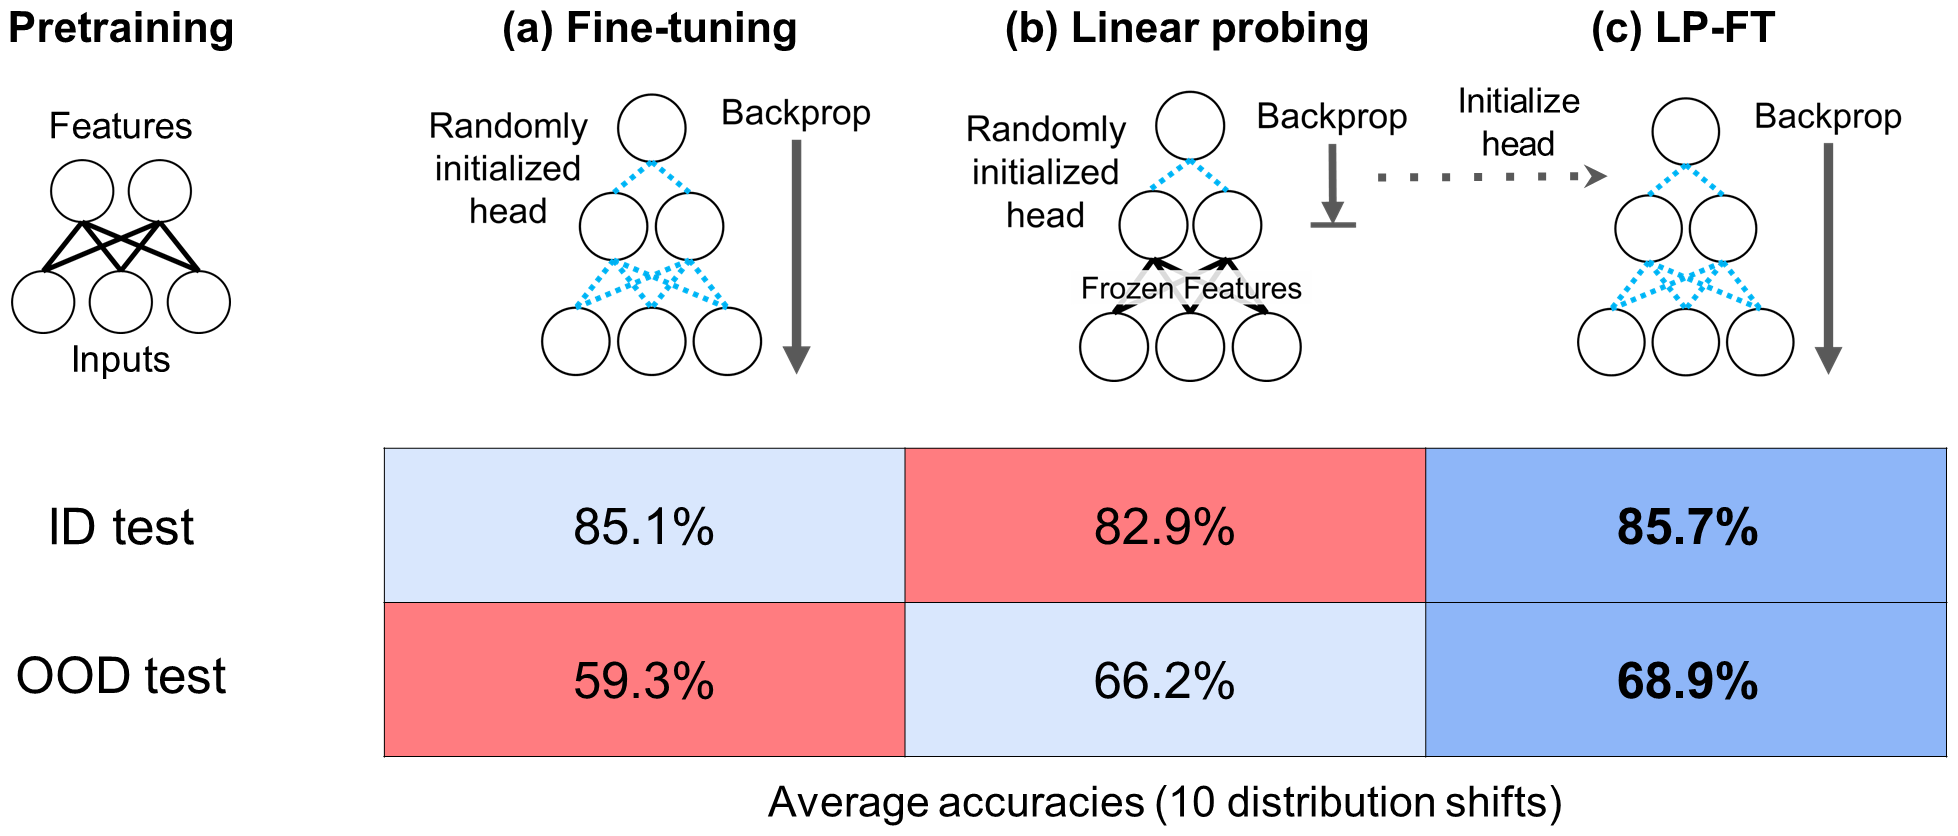
\includegraphics[width=\linewidth,height=0.44\textheight,keepaspectratio]{images/image-recognition/lpft_fig1_ft_lp_lpft_accuracy.png}\\[0.2em]
      {\scriptsize Kumar et al., ``Fine-Tuning can Distort Pretrained Features and Underperform Out-of-Distribution,'' ICLR 2022, \href{https://arxiv.org/abs/2202.10054v1}{arXiv:2202.10054v1}, Figure~1.\par}
      \vspace{0.4em}
      {\scriptsize\setlength{\tabcolsep}{3pt}
      \begin{tabular}{l c c c c c}
        \toprule
         & & \multicolumn{4}{c}{ImageNet shifts} \\
        \cmidrule(lr){3-6}
        ViT-B/16 & IN & V2 & R & Sketch & A \\
        \midrule
        FT & 81.7 & 71.5 & 52.4 & 40.5 & 27.8 \\
        LP & 79.7 & 69.7 & 70.6 & 46.4 & 45.7 \\
        LP-FT & 81.7 & 71.6 & 72.9 & 48.4 & 49.1 \\
        \bottomrule
      \end{tabular}\par}
      {\scriptsize CLIP ViT-B/16 trained on ImageNet, top-1 (\%). Same paper, Tables~1 and~2.\par}
  \end{columns}
\end{frame}

\begin{frame}{WiSE-FT: Weight-Space Ensembling}
  \begin{columns}[T,onlytextwidth]
    \column{0.52\textwidth}
      \begin{itemize}\footnotesize\itemsep0.3em
        \item \textbf{WiSE-FT} (weight-space ensembles for fine-tuning): fine-tune CLIP end-to-end, starting from its zero-shot head, then interpolate the weights:
          \[ \theta_\alpha = (1-\alpha)\,\theta_0 + \alpha\,\theta_1 \]
          $\theta_0$: zero-shot weights, with the head built from the class prompts; $\theta_1$: fine-tuned weights; $\alpha \in [0,1]$: mixing coefficient.
        \item Averaging two networks trained from random initialisations is no better than a random classifier. These two share the pretrained start, and accuracy stays high along the line between them.
        \item One network at test time, so inference costs the same as FT. Changing $\alpha$ needs no retraining; the authors recommend $\alpha = 0.5$ when nothing else is known.
        \item If only the head is fine-tuned, the encoder is shared and the interpolation equals output ensembling of the two models (covered earlier).
      \end{itemize}
    \column{0.46\textwidth}
      \centering
      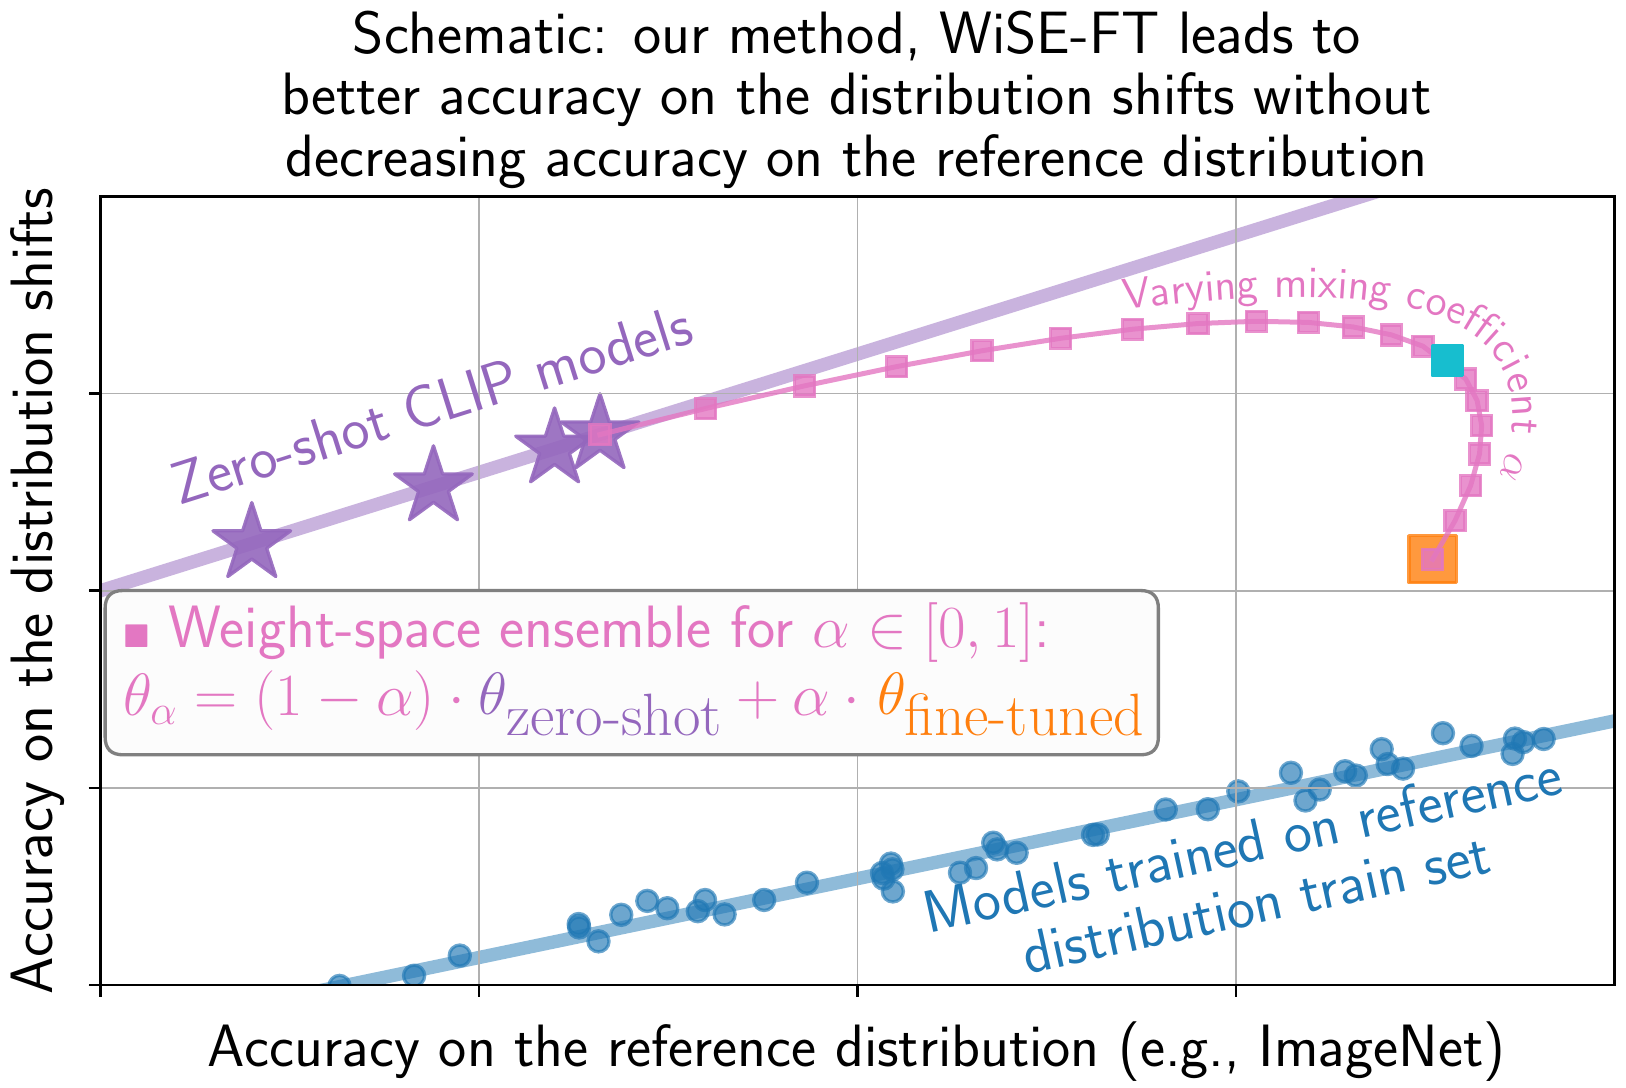
\includegraphics[width=\linewidth,height=0.58\textheight,keepaspectratio]{images/image-recognition/wiseft_fig1_weight_space_ensemble.png}\\[0.2em]
      {\scriptsize Schematic (top-right panel). Wortsman et al., \href{https://arxiv.org/abs/2109.01903v3}{arXiv:2109.01903v3}, Figure~1.\par}
      \vspace{0.4em}
      {\scriptsize\setlength{\tabcolsep}{4pt}
      \begin{tabular}{l c c}
        \toprule
        CLIP ViT-L/14@336px & IN & Mean, 5 shifts \\
        \midrule
        Zero-shot ($\alpha = 0$) & 76.6 & 73.4 \\
        Fine-tuned ($\alpha = 1$) & 86.2 & 68.6 \\
        WiSE-FT ($\alpha = 0.5$) & 86.8 & 76.9 \\
        \bottomrule
      \end{tabular}\par}
      {\scriptsize Top-1 (\%). Same paper, Table~1.\par}
  \end{columns}
\end{frame}

\begin{frame}{Model Soups: Averaging Many Fine-Tuned Models}
  \begin{columns}[T,onlytextwidth]
    \column{0.52\textwidth}
      \begin{itemize}\footnotesize\itemsep0.3em
        \item A hyperparameter sweep fine-tunes $k$ models $\theta_1,\dots,\theta_k$ from the same pretrained weights; usually only the best one on held-out data is kept.
        \item \textbf{Model soup:} average their weights instead. Uniform soup: $\theta_S = \frac{1}{k}\sum_{i=1}^{k}\theta_i$, where $\theta_S$ are the soup's weights. WiSE-FT with $\alpha = 0.5$ is a two-model uniform soup.
        \item \textbf{Greedy soup}, scored on a held-out split:
          \begin{enumerate}\footnotesize\itemsep0.05em
            \item sort the models by held-out accuracy, best first;
            \item start the soup with the best model;
            \item add each next model if the soup's held-out accuracy does not drop.
          \end{enumerate}
        \item Runs from one pretrained start tend to share a low-error basin. Runs with high learning rates can leave it and spoil a uniform soup; the greedy rule rejects them.
      \end{itemize}
    \column{0.46\textwidth}
      {\centering\scriptsize\setlength{\tabcolsep}{3pt}
      \begin{tabular}{l c c c}
        \toprule
        CLIP ViT-B/32, $k = 72$ & IN & Shifts & Passes \\
        \midrule
        Best single model\textsuperscript{*} & 80.38 & 47.83 & 1 \\
        Uniform soup & 79.97 & 51.45 & 1 \\
        Greedy soup (5 models) & 81.03 & 50.75 & 1 \\
        Output ensemble & 81.19 & 50.77 & $k$ \\
        \bottomrule
      \end{tabular}\par}
      \vspace{0.2em}
      {\scriptsize Top-1 (\%); Shifts: mean of the five ImageNet shifts; Passes: forward passes per image; \textsuperscript{*}picked by ImageNet accuracy. Wortsman et al., ``Model soups: averaging weights of multiple fine-tuned models improves accuracy without increasing inference time,'' ICML 2022, \href{https://arxiv.org/abs/2203.05482v3}{arXiv:2203.05482v3}, Table~3.\par}
      \begin{itemize}\footnotesize\itemsep0.3em
        \item Output ensembling (covered earlier) edges out the greedy soup on ImageNet but needs $k$ forward passes; the soup needs one.
        \item \textbf{ImageNet:} a greedy soup of 14 of 58 fine-tuned ViT-G/14 models reached 90.94\% top-1, above the best single model (90.72\%) and the previous state of the art (90.88\%).
      \end{itemize}
  \end{columns}
\end{frame}

\begin{frame}{Learned Prompts: CoOp and CoCoOp}

  {\centering
  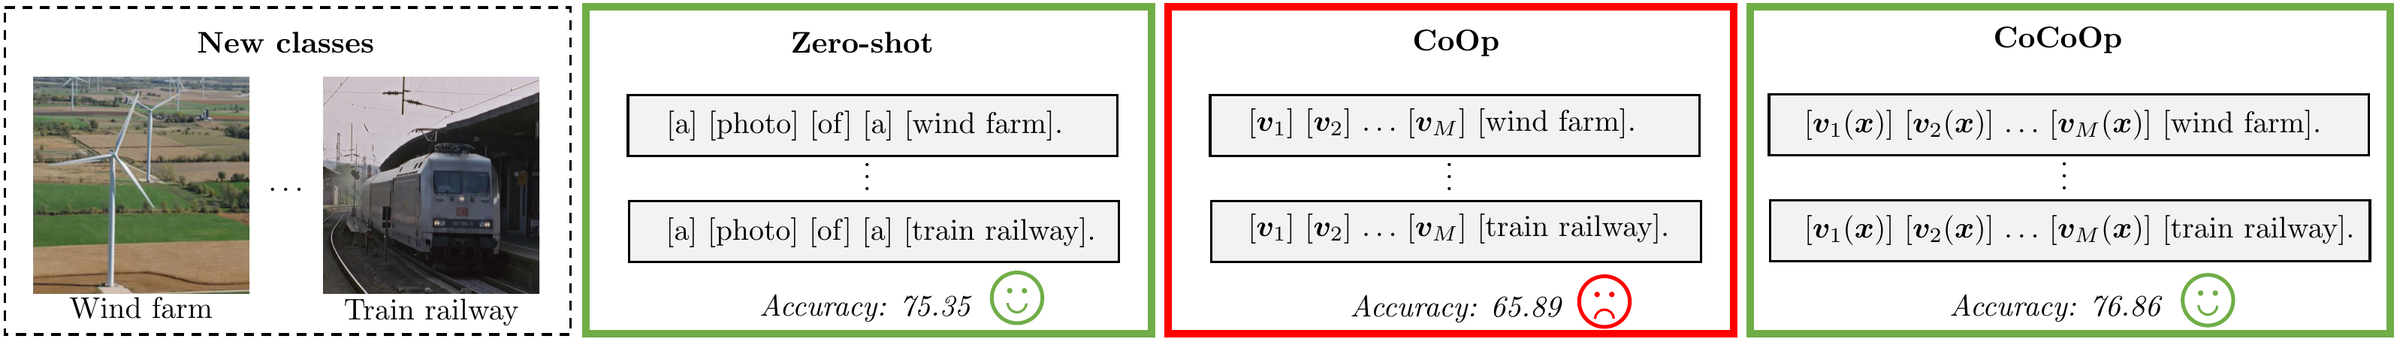
\includegraphics[width=0.88\textwidth,height=0.36\textheight,keepaspectratio]{images/image-recognition/cocoop_fig1b_new_class_prompts.png}\\[0.1em]
  {\scriptsize Prompts and accuracy (\%) on unseen classes of SUN397, a scene-recognition dataset. Zhou et al., ``Conditional Prompt Learning for Vision-Language Models,'' CVPR 2022, \href{https://arxiv.org/abs/2203.05557v2}{arXiv:2203.05557v2}, Figure~1(b).\par}}
  \vspace{0.3em}
  \begin{columns}[T,onlytextwidth]
    \column{0.52\textwidth}
      \begin{itemize}\footnotesize\itemsep0.2em
        \item \textbf{CoOp} (Context Optimization; Zhou et al., IJCV 2022) learns the context words of the prompt:
          \[ t_i = [\mathbf{v}_1][\mathbf{v}_2]\cdots[\mathbf{v}_M][\text{CLASS}_i] \]
          $\mathbf{v}_m$: learned vectors of word-embedding size, shared by all classes; $[\text{CLASS}_i]$: name of class $i$. Only the $\mathbf{v}_m$ are trained, with cross-entropy on a few labelled images; CLIP stays frozen.
        \item \textbf{CoCoOp} (Conditional Context Optimization): a two-layer network, Meta-Net, maps the image feature to a token $\boldsymbol{\pi}$; each context vector becomes $\mathbf{v}_m(\mathbf{x}) = \mathbf{v}_m + \boldsymbol{\pi}$.
      \end{itemize}
    \column{0.46\textwidth}
      {\centering\scriptsize\setlength{\tabcolsep}{3pt}
      \begin{tabular}{l c c c}
        \toprule
        Mean of 11 datasets & Base & New & H \\
        \midrule
        Zero-shot CLIP & 69.34 & 74.22 & 71.70 \\
        CoOp & 82.69 & 63.22 & 71.66 \\
        CoCoOp & 80.47 & 71.69 & 75.83 \\
        \bottomrule
      \end{tabular}\par}
      \vspace{0.2em}
      {\scriptsize ViT-B/16, 16 images per base class. Prompts are learned on half of each dataset's classes (base) and tested on base and on unseen (new) classes. H $= 2\cdot\text{Base}\cdot\text{New}/(\text{Base}+\text{New})$, the harmonic mean. Same paper, Table~1(a).\par}
      \begin{itemize}\scriptsize\itemsep0.2em
        \item The prompt depends on the image, so the text encoder runs for every image and class; training is slow (batch size 1). On 7 of the 11 datasets, CoCoOp stays below CLIP on new classes.
      \end{itemize}
  \end{columns}
\end{frame}

\begin{frame}{Tip-Adapter: A Training-Free Few-Shot Cache}

  {\centering
  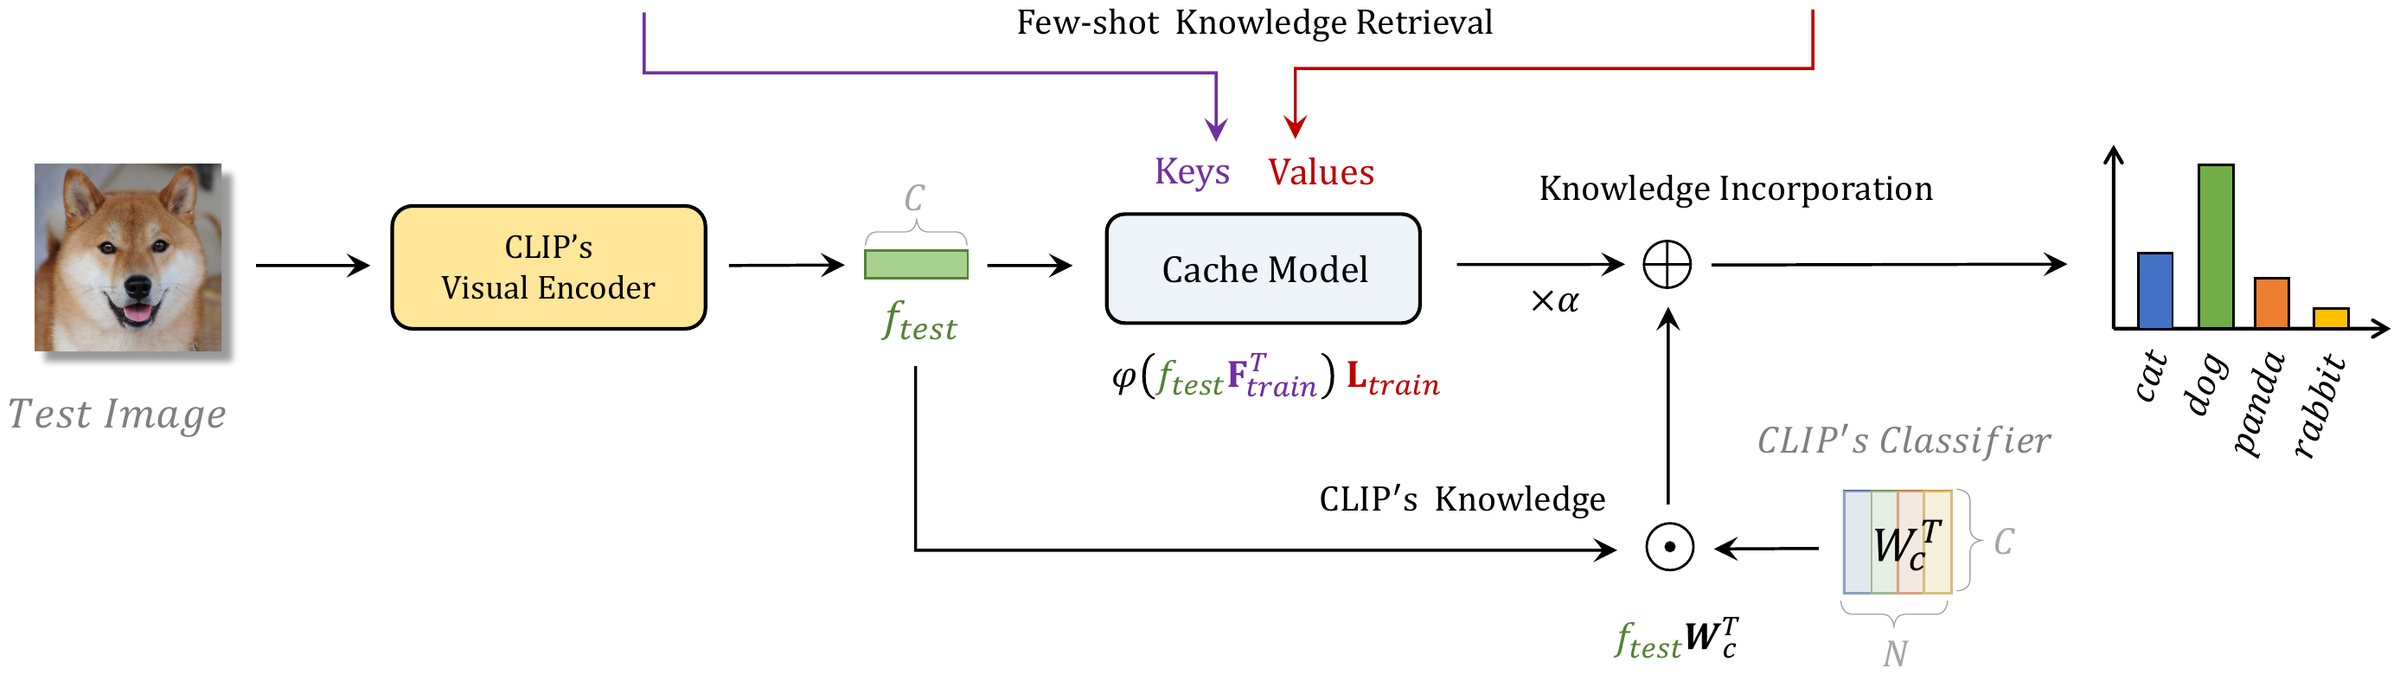
\includegraphics[width=\textwidth,height=0.34\textheight,keepaspectratio]{images/image-recognition/tipadapter_fig1_bottom_cache_inference.png}\\[0.1em]
  {\scriptsize Inference path (lower part of the figure). Zhang et al., ``Tip-Adapter: Training-free Adaption of CLIP for Few-shot Classification,'' ECCV 2022, \href{https://arxiv.org/abs/2207.09519v1}{arXiv:2207.09519v1}, Figure~1.\par}}
  \vspace{0.2em}
  \begin{columns}[T,onlytextwidth]
    \column{0.52\textwidth}
      \begin{itemize}\scriptsize\itemsep0.2em
        \item \textbf{Cache} from $K$ labelled images in each of $N$ classes: keys $\mathbf{F}_{\text{train}} \in \mathbb{R}^{NK\times C}$ are their L2-normalised CLIP features, values $\mathbf{L}_{\text{train}} \in \mathbb{R}^{NK\times N}$ their one-hot labels.
        \item For a test feature $f_{\text{test}} \in \mathbb{R}^{1\times C}$ (L2-normalised):
          \[ \begin{aligned} A &= \exp\!\big(-\beta\,(1 - f_{\text{test}}\mathbf{F}_{\text{train}}^{\top})\big)\\ \text{logits} &= \alpha\,A\,\mathbf{L}_{\text{train}} + f_{\text{test}}W_c^{\top} \end{aligned} \]
          $f_{\text{test}}\mathbf{F}_{\text{train}}^{\top}$: cosine similarities to the cached images; $\beta$: sharpness; $\alpha$: weight of the cache term; $W_c$: CLIP's zero-shot classifier.
      \end{itemize}
    \column{0.46\textwidth}
      \begin{itemize}\scriptsize\itemsep0.2em
        \item $A\,\mathbf{L}_{\text{train}}$: an affinity-weighted vote of the cached labels, a soft $k$-NN (covered earlier); the same lookup drives retrieval later in this lecture.
        \item \textbf{Tip-Adapter-F} (fine-tuned) trains only the keys, for 20 epochs against CoOp's 200. Top-1 (\%), Tables~1 and~5 (\textsuperscript{\textdagger}as Tip-Adapter reports it):
      \end{itemize}
      {\centering\scriptsize\setlength{\tabcolsep}{3pt}
      \begin{tabular}{l c c c}
        \toprule
        16 shots, ResNet-50 & IN & IN-V2 & IN-Sketch \\
        \midrule
        Zero-shot CLIP & 60.33 & 53.27 & 35.44 \\
        CoOp\textsuperscript{\textdagger} & 62.95 & 54.58 & 31.04 \\
        Tip-Adapter & 62.03 & 54.60 & 35.90 \\
        Tip-Adapter-F & 65.51 & 57.11 & 36.00 \\
        \bottomrule
      \end{tabular}\par}
  \end{columns}
\end{frame}

\begin{frame}{Classification by LLM-Written Descriptions}

  {\centering
  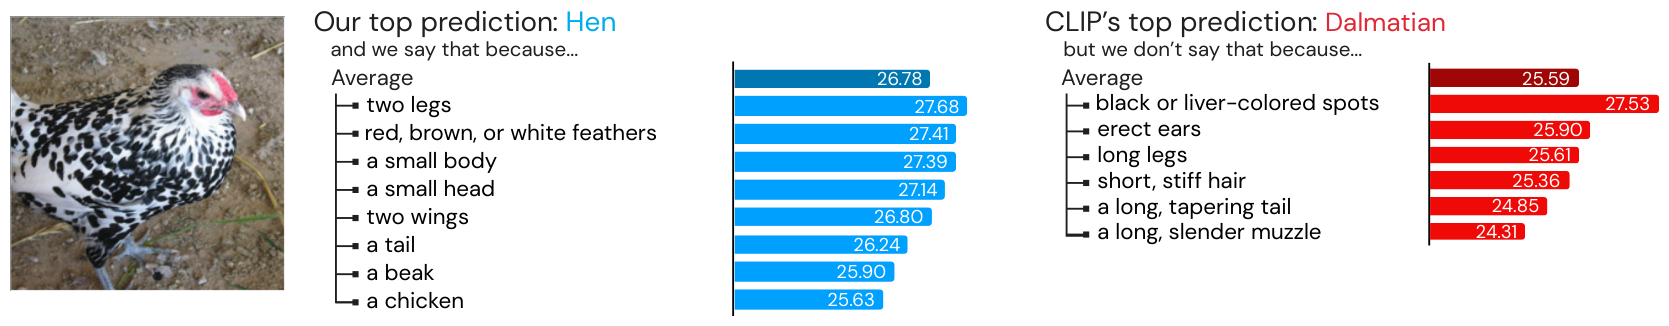
\includegraphics[width=\textwidth,height=0.38\textheight,keepaspectratio]{images/image-recognition/classbydesc_fig1_hen_explanation.png}\\[0.1em]
  {\scriptsize Descriptor scores behind ``hen'' (left) and the lower scores for ``Dalmatian'', CLIP's wrong answer (right). Menon and Vondrick, ``Visual Classification via Description from Large Language Models,'' ICLR 2023, \href{https://openreview.net/forum?id=jlAjNL8z5cs}{OpenReview}, Figure~1.\par}}
  \vspace{0.2em}
  \begin{columns}[T,onlytextwidth]
    \column{0.52\textwidth}
      \begin{itemize}\scriptsize\itemsep0.2em
        \item \textbf{Descriptors:} a large language model (LLM), GPT-3 in the paper, is asked ``What are useful features for distinguishing a \{category name\} in a photo?'' Its list is the descriptor set $D(c)$ of class $c$.
        \item \textbf{Score:} CLIP compares the image $\mathbf{x}$ with each text ``\{category\_name\} which (is/has/etc) \{descriptor\}'':
          \[ s(c,\mathbf{x}) = \frac{1}{|D(c)|}\sum_{d \in D(c)} \phi(d,\mathbf{x}) \]
          $\phi(d,\mathbf{x})$: CLIP similarity of descriptor $d$ and image $\mathbf{x}$. The predicted class is $\operatorname*{arg\,max}_{c}\, s(c,\mathbf{x})$.
      \end{itemize}
    \column{0.46\textwidth}
      \begin{itemize}\scriptsize\itemsep0.2em
        \item No training. The descriptor scores explain each decision, and editing $D(c)$ edits the classifier.
        \item Table~1: ImageNet top-1 from 58.46\% to 62.97\% (ViT-B/32) and from 72.97\% to 76.16\% (ViT-L/14@336px); ImageNetV2 from 66.58\% to 70.32\% (ViT-L/14@336px). The baseline is CLIP with the bare class name.
        \item \textbf{CuPL} (Customized Prompts via Language models; Pratt et al., ICCV 2023) uses LLM-written sentences as prompts: 76.69\% on ImageNet vs 75.54\% for CLIP's 80 hand-written templates (ViT-L/14, Table~1).
      \end{itemize}
  \end{columns}
\end{frame}

\begin{frame}{Adaptation Recipes Side by Side}
  \footnotesize
  Numbers from the earlier slides of this section (top-1, \%; shifts: mean over the shifted test sets).
  \vspace{0.3em}

  {\centering\scriptsize\setlength{\tabcolsep}{4pt}
  \begin{tabular}{>{\raggedright\arraybackslash}p{1.6cm} >{\raggedright\arraybackslash}p{2.4cm} >{\raggedright\arraybackslash}p{2.0cm} >{\raggedright\arraybackslash}p{2.1cm} >{\raggedright\arraybackslash}p{4.1cm}}
    \toprule
    \textbf{Recipe} & \textbf{What is trained} & \textbf{Labels} & \textbf{Test-time cost} & \textbf{Evidence (method vs baseline)} \\
    \midrule
    FT & all weights & full training set & one network & IN 86.2 vs 76.6, shifts 68.6 vs 73.4 (zero-shot) \\
    LP-FT & head, then all weights & full training set & one network & 10-shift OOD 68.9 vs 59.3 (FT) \\
    WiSE-FT & FT, then interpolation with $\theta_0$ & full training set & one network & shifts 76.9 vs 68.6, IN 86.8 vs 86.2 (FT) \\
    Greedy soup & $k$ FT runs, averaged & full set, with a held-out split & one network & shifts 50.75 vs 47.83, IN 81.03 vs 80.38 (best single model by ImageNet accuracy) \\
    CoOp & $M$ context vectors & 16 per base class & fixed prompts & new classes 63.22 vs 74.22 (CLIP) \\
    CoCoOp & context vectors and Meta-Net & 16 per base class & prompts per image & new classes 71.69 vs 74.22, H 75.83 vs 71.70 (CLIP) \\
    Tip-Adapter & nothing & 16 per class & two extra matrix products & IN 62.03 vs 60.33 (zero-shot CLIP) \\
    Descriptions & nothing & none & one score per descriptor & IN-V2 70.32 vs 66.58 (class name only) \\
    \bottomrule
  \end{tabular}\par}
\end{frame}
